\subsection{Meteors Databases}
\label{ssec:databases}
We selected a sample of meteors which were observed in mexican territory from the Geostationary Lightning Mapper \citep{GOODMAN:2013}. Orignally this project was designed to detect ligthning activity in earth's athmosphere, but has been proven that also can detect bolides entering the athmosphere. The detection comes from two satellites called GOES-16 and GOES-17 orbiting the earth in geostationary orbits. %Figure  shows the area where GOES-16 and GOES-17 detect activity on a lightning flash rate map; in mexican territory clearly both satellites can make detections. %Create a figure where the area coverage of GOES-16 and GOES-17 is shown.
We used the interactive database available at \url{https://neo-bolide.ndc.nasa.gov/#/}. These data are publicly available and easily downloaded from the same website. For each event we can obtain the recorded trajectory of meteors and the corresponding light curve. THe GLM satellites have an umbral magnitude for detection of -14. At this magnitude, a meteor is considered a bolide, and is expected to be at least decimeter-sized (in diameter) to reach such brightness. In the other hand, too bright meteors will saturate the detectors, and thus, lowering the quality of data. The result of this factors implies that the range in size of the objects in our sample varies in diameter between decimeter to meter size. %The sample was chosen following the next criteria:%selected in such way we chose the most probable objects to be detected by GPS sources in mexican territory and its surroundings: 
Each event also has assigned a confidence ratio, from low confidence to high, depending in how bright is the event itself and if the trajectory recorded by GLM ressembles (or not) a straight line. We chose only events whose confidence ratio is high, in oreder to be sure we chose the brightest objects, and thus, in the diameter size of bolides, we favored the meter-sized ones. In table \ref{tab:table-meteors} we list the object we chose to do this work, order in chronological order. The columns of the table, from left to right are and ID to enumerate the meteors in the sample, the date and time each meteor was detected, the duration of the detection, their respective coordinates and the estimated height of the meteor over the ground at the time of the detection. GOES-16 and GOES-17 systematically detect the meteors at slightly different positions and at slightly different times, so we calculated the mean of the duration, latitude and longitude reported by both satellites for each event, and used the standard deviation as the uncertainties.

From table \ref{tab:table-meteors} is also clear that the duration of all the bolides detection last less than a second. This obsevation suggests that the bolides remain undetected by the GLM satellites until they get fragmented due to stagnation presure when they release a huge amount of energy and thus they become detectable.

%From the light curves we can estimate the total radiated energy and then convert it to the total kinetic energy through a relation. With this energy we may estimate physical parameters with the cloud fragmentation model form wheeler et al.

%\begin{itemize}
%    \item The objects were detected inside mexican territory and its surroundings.
%    \item The objects were detected by both satellites GOES 16 and GOES 17 (stereo)
%    \item The detection has been assigned a high confidence ratio.
%\end{itemize}



\begin{table*}
  \centering
  \footnotesize
  \caption{List of meteors passing through Mexico. The events are listed in chronological order. The listed duration, latitude and longitude correspond to the mean of the measurements of both GOES satellites. The uncertainties correspond to the respecting mean deviation.}
\label{tab:table-meteors}
\begin{tabular}{rrrrrrrrr}
\hline
ID & Date of event  & Start Time (UT)  & Duration (seconds) & Latitude (deg) & Longitude (deg)& Altitude (km)\\\hline
GLM-00 & 2019-02-01 & 18:17:09 & $2.651\pm 0.4907$ & $22.45 \pm 0.071$ & $-83.50  \pm  0.424$ & 24           \\         
GLM-01 & 2019-05-23 & 16:36:18 & $0.197\pm 0.0000$ & $24.30 \pm 0.000$ & $-101.60 \pm  0.849$ & 28           \\
GLM-02 & 2019-07-18 & 14:30:30 & $0.058\pm 0.0000$ & $27.20 \pm 0.000$ & $-103.15 \pm  0.778$ & 72           \\
GLM-03 & 2019-08-10 & 11:18:48 & $0.199\pm 0.0757$ & $21.50 \pm 0.000$ & $-102.50  \pm 0.849$ & 92           \\
GLM-04 & 2019-10-03 & 07:55:33 & $0.106\pm 0.0297$ & $25.65 \pm 0.071$ & $-96.25 \pm   0.778$ & 74           \\
GLM-05 & 2019-10-09 & 06:08:11 & $0.103\pm 0.0078$ & $23.60 \pm 0.000$ & $-111.95 \pm  0.212$ & 32           \\
GLM-06 & 2019-11-16 & 09:36:04 & $0.396\pm 0.0134$ & $20.30 \pm 0.000$ & $-100.55 \pm  0.919$ & 82           \\
GLM-07 & 2019-11-17 & 15:36:01 & $0.116\pm 0.0035$ & $31.70 \pm 0.000$ & $-117.70 \pm  1.131$ & 88           \\
GLM-08 & 2019-11-19 & 07:57:40 & $0.097\pm 0.1138$ & $20.00 \pm 0.000$ & $-88.40 \pm   1.131$ & 99           \\
GLM-09 & 2019-11-26 & 13:23:20 & $0.078\pm 0.0290$ & $23.90 \pm 0.000$ & $-108.70 \pm  0.849$ & 81           \\
GLM-10 & 2019-12-04 & 09:42:54 & $0.173\pm 0.0028$ & $31.50 \pm 0.000$ & $-113.65 \pm  0.919$ & 77           \\
GLM-11 & 2019-12-15 & 14:50:49 & $0.127\pm 0.0134$ & $27.70 \pm 0.000$ & $-114.10 \pm  0.849$ & 78           \\
GLM-12 & 2019-12-29 & 16:16:35 & $0.062\pm 0.0134$ & $29.60 \pm 0.000$ & $-116.35 \pm  0.919$ & 79           \\
GLM-13 & 2020-01-03 & 14:10:17 & $0.113\pm 0.0085$ & $30.20 \pm 0.000$ & $-117.65 \pm  0.919$ & 74           \\
GLM-14 & 2020-01-06 & 16:39:27 & $0.118\pm 0.0042$ & $31.40 \pm 0.000$ & $-108.20 \pm  0.990$ & 81           \\
GLM-15 & 2020-01-15 & 15:00:33 & $0.213\pm 0.1351$ & $19.45 \pm 0.071$ & $-95.55 \pm   0.919$ & 93           \\
GLM-16 & 2020-02-12 & 09:25:40 & $0.210\pm 0.0226$ & $18.90 \pm 0.000$ & $-93.50 \pm   0.849$ & 90           \\
GLM-17 & 2020-03-03 & 12:33:27 & $0.062\pm 0.0007$ & $18.25 \pm 0.071$ & $-106.35 \pm  0.636$ & 77           \\
GLM-18 & 2020-03-31 & 19:31:52 & $0.105\pm 0.0573$ & $28.45 \pm 0.071$ & $-112.05 \pm  0.636$ & 61           \\
GLM-19 & 2020-04-08 & 16:25:28 & $0.120\pm 0.0926$ & $26.10 \pm 0.000$ & $-93.90 \pm   0.849$ & 78           \\
GLM-20 & 2020-04-18 & 17:43:25 & $0.139\pm 0.0106$ & $29.00 \pm 0.000$ & $-106.55 \pm  0.919$ & 82           \\
GLM-21 & 2020-04-20 & 16:05:22 & $0.318\pm 0.1655$ & $28.15 \pm 0.071$ & $-97.85 \pm   1.061$ & 88           \\
GLM-22 & 2020-04-25 & 11:03:09 & $0.323\pm 0.0813$ & $32.15 \pm 0.071$ & $-111.60 \pm  1.131$ & 84           \\
GLM-23 & 2020-04-28 & 19:31:52 & $0.105\pm 0.0573$ & $28.45 \pm 0.071$ & $-112.05 \pm  0.636$ & 29           \\
GLM-24 & 2020-05-08 & 10:06:16 & $0.490\pm 0.0750$ & $21.60 \pm 0.000$ & $-92.40 \pm   0.849$ & 81           \\
GLM-25 & 2020-07-15 & 19:58:28 & $0.693\pm 0.0495$ & $24.00 \pm 0.000$ & $-108.35 \pm  0.495$ & 53           \\
GLM-26 & 2020-08-07 & 13:29:57 & $0.163\pm 0.0057$ & $28.80 \pm 0.000$ & $-106.05 \pm  0.919$ & 89           \\
GLM-27 & 2020-09-13 & 16:41:59 & $0.184\pm 0.0078$ & $28.45 \pm 0.071$ & $-113.75 \pm  0.919$ & 85           \\
GLM-28 & 2020-09-30 & 12:28:11 & $0.100\pm 0.0078$ & $24.90 \pm 0.000$ & $-110.90 \pm  0.849$ & 83           \\
GLM-29 & 2020-11-16 & 12:28:11 & $0.100\pm 0.0078$ & $24.90 \pm 0.000$ & $-110.90 \pm  0.849$ &106           \\
GLM-30 & 2020-11-17 & 12:53:41 & $0.404\pm 0.0262$ & $23.00 \pm 0.000$ & $-102.45 \pm  0.919$ & 93           \\
GLM-31 & 2020-12-19 & 10:18:14 & $0.407\pm 0.0110$ & $21.95 \pm 0.071$ & $-101.60 \pm  0.990$ & 98           \\
GLM-32 & 2020-12-23 & 09:43:01 & $0.148\pm 0.0014$ & $25.75 \pm 0.071$ & $-111.25 \pm  0.778$ & 81           \\
GLM-33 & 2020-12-29 & 15:20:54 & $0.118\pm 0.0014$ & $16.80 \pm 0.000$ & $-102.20 \pm  0.707$ & 81           \\
GLM-34 & 2021-03-31 & 09:01:17 & $0.753\pm 0.3083$ & $20.15 \pm 0.071$ & $-92.95 \pm  0.212$  & 24           \\
GLM-Ven& 2019-06-22 & 21:25:45 & $4.873\pm 0.0000$ & $14.9 \pm 0.000$  & $-65.8 \pm 0.000$    & 25           \\ \hline
\end{tabular}
\end{table*}

\begin{figure}
  \centering
  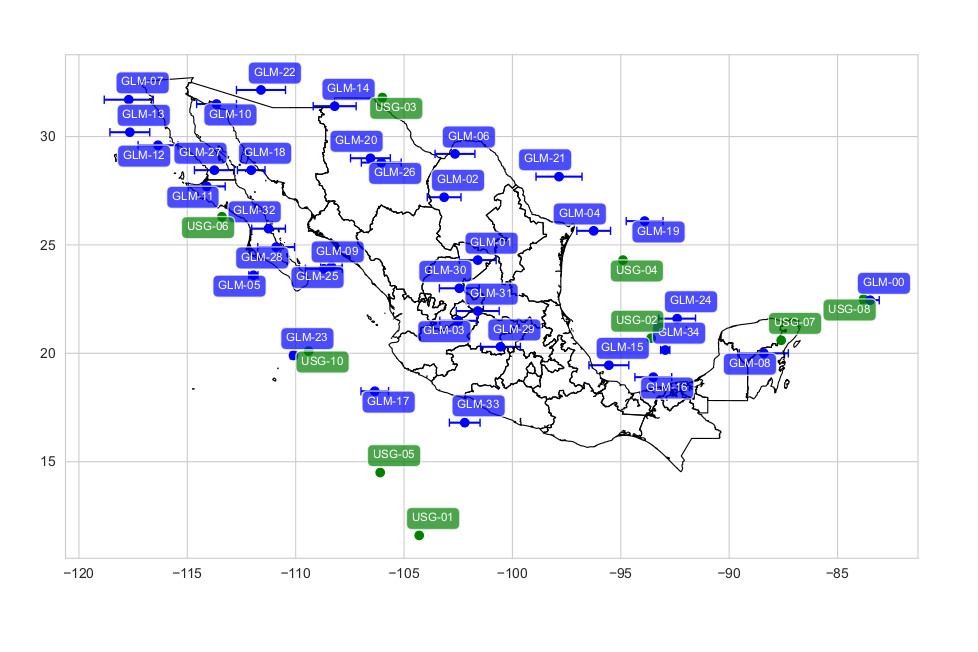
\includegraphics[width=\linewidth]{../meteors_map}
  \caption{Positions of events from table \ref{tab:table-meteors}. The label of each point correspond to the ID (first column) of the referred table.}
  \label{fig:meteors-map}
\end{figure}

By the other hand, we got another sample from USG sensors from the Center for Near Earth Object Studies (CNEOS), publicly available at \url{https://cneos.jpl.nasa.gov/fireballs/}. As seen in table  , the time span is quite larger, and the released energy is generally larger, as seen in figure  . Some elements appear in both samples, since are bright enough to be detected regardless the project involved. In USG sample, the total energy of each meteor is obtained directly, but is nt the case for the GLM sample. In appendix  we give details about how the total energy is obtained.

\begin{table*}
    \centering
  \footnotesize
  \caption{List of meteors passing through Mexico. The events are listed in chronological order. The listed duration, latitude and longitude correspond to the mean of the measurements of both GOES satellites. The uncertainties correspond to the respecting mean deviation.}
\label{tab:table-meteors}
\begin{tabular}{rrrrrrrrrr}
       &               &                  & \multicolumn{4}{c}{Velocity (km/s)}       &                   &                 &\\\cline{4-7}
\multicolumn{1}{c}{ID}&\multicolumn{1}{c}{Date of event}&\multicolumn{1}{c}{Start Time (UT)}&\multicolumn{1}{c}{$v$}&\multicolumn{1}{c}{$v_x$}&\multicolumn{1}{c}{$v_y$}&\multicolumn{1}{c}{$v_z$}&\multicolumn{1}{c}{Latitude (deg)}&\multicolumn{1}{c}{Longitude (deg)}&\multicolumn{1}{c}{Altitude (km)}\\\hline
USG-01 & 1995-08-05    & 17:14:10         &      &         &           &              & 11.6              &  -104.3         &             \\
USG-02 & 1996-07-12    & 14:04:45         &      &         &           &              & 20.7              &   -93.6         &             \\ 
USG-03 & 1997-10-09    & 18:47:15         &      &         &           &              & 31.8              &  -106.0         &   37.0      \\
USG-04 & 2000-01-18    & 08:33:58         &      &         &           &              & 24.3              &   -94.9         &             \\
USG-05 & 2000-08-25    & 01:12:25         &      &         &           &              & 14.5              &  -106.1         &             \\
USG-06 & 2005-11-15    & 05:19:07         &      &         &           &              & 26.3              &  -113.4         &   32.4      \\
USG-07 & 2015-07-19    & 07:06:26         & 17.8 &   9.4   &  13.0     & 7.8          & 20.6              &   -87.6         &   22.0      \\
USG-08 & 2019-02-01    & 18:17:10         & 16.3 &  -2.4   &  13.6     & 8.7          & 22.5              &   -83.8         &   23.7      \\
USG-09 & 2019-06-22    & 21:25:48         & 14.9 & -13.4   &   6.0     & 2.5          & 14.9              &   -66.2         &   25.0      \\
USG-10 & 2020-04-28    & 05:43:17         &      &         &           &              & 20.1              &  -109.4         &             \\\hline  
  \end{tabular}
\end{table*}

  
\subsection{GPS data}
\label{ssec:GPS}
This material is based on services provided by the GAGE Facility, operated by UNAVCO, Inc., with support from the National Science Foundation and the National Aeronautics and Space Administration under NSF Cooperative Agreement EAR-1724794.

We got RINEX data from 3 to 7 stations depending of the event location and data availability that surround the event place in all directions as possible. A list of the stations where we got RINEX data is available in table \ref{tab:table-stations}. Most of the stations lie in mexican territory, but in some cases we required data from other stations to cover events near the mexican frontier at north or south.

\clearpage
\onecolumn
\footnotesize
\begin{landscape}
%\begin{table*}
%    \centering
  \begin{longtable}{llllllp{12cm}}
      \caption{List of GPS stations used for this work.}
      \label{tab:table-stations}
      \endfirsthead
      \endhead
    \hline
    Station name & Latitude & Longitude & \multicolumn{3}{c}{Events ID}  & Citation \\\hline
    \multirow{4}{*}{BAR1\hyperlink{Hudnut}{${}^1$}\hyperlink{Hudnut2}{${}^5$}} & \multirow{4}{*}{33.48} & \multirow{4}{*}{-119.03} & \multirow{4}{*}{GLM-07} & \multirow{4}{*}{GLM-12} & \multirow{4}{*}{GLM-13} & UNAVCO Community, Hudnut, Kenneth, King, Nancy, Aspiotes, Aris G., Borsa, Adrian A., Determan, \\
    &&&&&& Daniel N., Galetzka, John E., Stark, Keith F., 2005, SCIGN-PBO Nucleus GPS Network - BAR1-Santa \\
    &&&&&& Barbara Island One P.S., The GAGE Facility operated by UNAVCO, Inc., GPS/GNSS Observations Dataset, \\
    &&&&&& \url{https://doi.org/10.7283/T5668BHN}.\\\hline
    \multirow{3}{*}{BLYT\hyperlink{Hudnut}{${}^1$}} & \multirow{3}{*}{33.61} & \multirow{3}{*}{-114.71} &  \multirow{3}{*}{GLM-12} & \multirow{3}{*}{GLM-13}  & & Hudnut, Kenneth, King, Nancy, Aspiotes, Aris G., Borsa, Adrian A., Determan, Daniel N., Galetzka, John \\
    &&&&&& E., Stark, Keith F., 2006, SCIGN USGS GPS Network - BLYT-Blythe P.S., The GAGE Facility operated \\
    &&&&&&  by UNAVCO, Inc., GPS/GNSS Observations Dataset, \url{https://doi.org/10.7283/T5HT2MKK}.\\\hline
    \multirow{3}{*}{CN23} & \multirow{3}{*}{17.26} & \multirow{3}{*}{-88.78} &\multirow{3}{*}{GLM-08} & \multirow{3}{*}{GLM-15} & \multirow{3}{*}{GLM-16} & UNAVCO Community, 2012, COCONet GPS Network - CN23-BelmopanBZCR2012 P.S., The GAGE \\
    &&&&&& Facility operated by UNAVCO, Inc., GPS/GNSS Observations Dataset, \\
    &&&&&& \url{https://doi.org/10.7283/T5Q23XJH}.\\\hline
    \multirow{3}{*}{CN25} & \multirow{3}{*}{16.23} & \multirow{3}{*}{-92.13} & \multirow{3}{*}{GLM-15} & & & UNAVCO Community, 2014, COCONet GPS Network - CN25-ComitandDMEX2012 P.S., The GAGE Facility operated by UNAVCO, Inc., GPS/GNSS Observations Dataset, \url{https://doi.org/10.7283/T57W69G7}.\\\hline
    \multirow{3}{*}{GCFS} & \multirow{3}{*}{19.31} & \multirow{3}{*}{-81.18} & \multirow{3}{*}{GLM-08} & & & Watts, Anthony, 2016, COCONet GPS Network - GCFS-G\_CAYMAN\_CYM2014 P.S., The GAGE Facility operated by UNAVCO, Inc., GPS/GNSS Observations Dataset, \url{https://doi.org/10.7283/7ETV-X536}.\\\hline
    \multirow{4}{*}{GMPK\hyperlink{Hudnut}{${}^1$}} & \multirow{4}{*}{33.05} & \multirow{4}{*}{-114.83} & \multirow{4}{*}{GLM-10} & & & UNAVCO Community, Hudnut, Kenneth, King, Nancy, Aspiotes, Aris G., Borsa, Adrian A., Determan, \\
    &&&&&& Daniel N., Galetzka, John E., Stark, Keith F., 2005, SCIGN-PBO Nucleus GPS Network - GMPK-Glamis \\
    &&&&&& Peak P.S., The GAGE Facility operated by UNAVCO, Inc., GPS/GNSS Observations Dataset, \\
    &&&&&& \url{https://doi.org/10.7283/WCHN-H687}.\\\hline
    \multirow{3}{*}{GUAT\hyperlink{Garnier}{${}^2$}} & \multirow{3}{*}{14.59} & \multirow{3}{*}{-90.52} & \multirow{3}{*}{GLM-16} & & & DeMets, Charles, Cosenza-Muralles, Beatriz, 2021, Central America 2018 - Guatemala, The GAGE \\
    &&&&&& Facility operated by UNAVCO, Inc., GPS/GNSS Observations Dataset, \\
    &&&&&& \url{https://doi.org/10.7283/KH2R-K704}.\\\hline
\multirow{4}{*}{GUAX\hyperlink{Hudnut}{${}^1$}} & \multirow{4}{*}{28.88} & \multirow{4}{*}{-118.29} & GLM-05 & GLM-07 & GLM-11 & Hudnut, Kenneth, King, Nancy, Aspiotes, Aris G., Borsa, Adrian A., Determan, Daniel N., Galetzka, John \\
    &&&GLM-12& GLM-13& GLM-18 & E., Stark, Keith F., 2001, SCIGN USGS GPS Network - GUAX-Isla Guadalupe P.S., The GAGE Facility \\
    &&& GLM-25 &GLM-27 &GLM-28& operated by UNAVCO, Inc., GPS/GNSS Observations Dataset, \url{https://doi.org/10.7283/T5GX48T2}.\\
    &&& GLM-32 &       &     &  \\\hline
    \multirow{3}{*}{IAGX} & \multirow{3}{*}{29.03} & \multirow{3}{*}{-113.17} & \multirow{3}{*}{GLM-10} & & & Gonzalez-Ortega, Alejandro, Galetzka, John E., Gonzalez, Javier, 2018, CICESE REGNOM GPS Network \\
    &&&&&& - IAGX-iagxREGNOMmx2018 P.S., The GAGE Facility operated by UNAVCO, Inc., GPS/GNSS  \\
    &&&&&& Observations Dataset, \url{https://doi.org/10.7283/DGWN-A627}. \\\hline
    \multirow{2}{*}{INEG} & \multirow{2}{*}{21.85} & \multirow{2}{*}{-102.28} & GLM-25 & GLM-26 & GLM-28  & No citations were found \\
    &&& GLM-29 & GLM-30 & GLM-31 & \\\hline 
    \multirow{4}{*}{KVTX} & \multirow{4}{*}{27.55} & \multirow{4}{*}{-97.89} & GLM-01 & GLM-02 & GLM-03  & UNAVCO Community, 2007, PBO GPS Network - KVTX-KingsvilleTX2006 P.S., The GAGE Facility \\
    &&& GLM-04 & GLM-06 & GLM-19 & operated by UNAVCO, Inc., GPS/GNSS Observations Dataset, \url{https://doi.org/10.7283/T5J38QH8}.\\
    &&& GLM-20 & GLM-21 & GLM-24 & \\
    &&& GLM-26 &&& \\\hline
    MDO1 & 30.68 & -104.02 & GLM-02 & & & No citations were found\\\hline
    MGO5 & 30.68 & -104.02 & GLM-21 &GLM-26 &  & No citations were found\\\hline
    MGW3 & 29.62 & -89.95 & GLM-19 & GLM-21 & GLM-24 & No citations were found\\\hline
    \multirow{3}{*}{OXTH} & \multirow{3}{*}{16.29} & \multirow{3}{*}{-95.24} & \multirow{3}{*}{GLM-15} & \multirow{3}{*}{GLM-16} & & DeMets, Charles, Cabral-Cano, Enrique, 2008, Oaxaca GPS Network - OXTH-Tehuantepec P.S., The \\
    &&&&&& GAGE Facility operated by UNAVCO, Inc., GPS/GNSS Observations Dataset, \\
    &&&&&& \url{https://doi.org/10.7283/T5Q81B5V}.\\\hline
    \multirow{3}{*}{OXUM\hyperlink{Graham}{${}^3$}} & \multirow{3}{*}{15.66} & \multirow{3}{*}{-96.50} & \multirow{3}{*}{GLM-34} & & & Cabral-Cano, Enrique, Salazar-Tlaczani, Luis, 2015, TLALOCNet - OXUM-oxum\_tnet\_mx2001 P.S., The \\
    &&&&&& GAGE Facility operated by UNAVCO, Inc., GPS/GNSS Observations Dataset, \\
    &&&&&& \url{https://doi.org/10.7283/T5J964RP}.\\\hline
    \multirow{2}{*}{P001} & \multirow{2}{*}{31.95} & \multirow{2}{*}{-112.80} & \multirow{2}{*}{GLM-07} & \multirow{2}{*}{GLM-22} & & UNAVCO Community, 2008, PBO GPS Network - P001-Organ\_PipeAZ2007 P.S., The GAGE Facility \\
    &&&&&& operated by UNAVCO, Inc., GPS/GNSS Observations Dataset, \url{https://doi.org/10.7283/T5DR2SGP}.\\\hline
    \multirow{2}{*}{P014} & \multirow{2}{*}{31.97} & \multirow{2}{*}{-11.09} & GLM-10 & GLM-12 & GLM-13 & UNAVCO Community, 2008, PBO GPS Network - P014-Sahuarita\_AZ2007 P.S., The GAGE Facility \\
    &&& GLM-14 & GLM-22 & & operated by UNAVCO, Inc., GPS/GNSS Observations Dataset, \url{https://doi.org/10.7283/T5DJ5CMK}.\\\hline
    \multirow{2}{*}{P807} & \multirow{2}{*}{30.49} & \multirow{2}{*}{-98.82} & GLM-06 & GLM-14 & GLM-21 & UNAVCO Community, 2012, PBO GPS Network - P807-EcRockStPkTX2012 P.S., The GAGE Facility \\
    &&& GLM-30 &&& operated by UNAVCO, Inc., GPS/GNSS Observations Dataset, \url{https://doi.org/10.7283/T5TQ5ZKM}.\\\hline
    \multirow{2}{*}{PLPX} & \multirow{2}{*}{31.59} & \multirow{2}{*}{-115.15} & \multirow{2}{*}{GLM-10} & & & UNAVCO Community, 2011, PBO GPS Network - PLPX-Las\_PintasMX2010 P.S., The GAGE Facility \\
    &&&&&& operated by UNAVCO, Inc., GPS/GNSS Observations Dataset, \url{https://doi.org/10.7283/T5K64G3T}.\\\hline
    \multirow{2}{*}{PTEX} & \multirow{2}{*}{32.29} & \multirow{2}{*}{-116.52} & GLM-07 & GLM-12 & GLM-13  & UNAVCO Community, 2011, PBO GPS Network - PTEX-Testerazo\_MX2011 P.S., The GAGE Facility \\
    &&& GLM-27 & GLM-32 & & operated by UNAVCO, Inc., GPS/GNSS Observations Dataset, \url{https://doi.org/10.7283/T5610XBP}.\\\hline 
    \multirow{3}{*}{RG06} & \multirow{3}{*}{32.63} & \multirow{3}{*}{-107.86} & \multirow{3}{*}{GLM-22} & & & Sheehan, Anne, 2007, Rio Grande Rift GPS Network - RG06-RG06FaywodNM2006 P.S., The GAGE \\
    &&&&&& Facility operated by UNAVCO, Inc., GPS/GNSS Observations Dataset, \\
    &&&&&& \url{https://doi.org/10.7283/T5668BFR}.\\\hline
    \multirow{3}{*}{RG07} & \multirow{3}{*}{32.50} & \multirow{3}{*}{-106.84} & \multirow{3}{*}{GLM-14} & & & Sheehan, Anne, 2007, Rio Grande Rift GPS Network - RG07-RG07CrucesNM2006 P.S., The GAGE  \\
    &&&&&& Facility operated by UNAVCO, Inc., GPS/GNSS Observations Dataset, \\
    &&&&&& \url{https://doi.org/10.7283/T5KD1W45}. \\\hline
    \multirow{3}{*}{SG33} & \multirow{3}{*}{31.77} & \multirow{3}{*}{-106.51} & \multirow{3}{*}{GLM-06} & \multirow{3}{*}{GLM-20} & \multirow{3}{*}{GLM-26} & Harder, Steven, Kaip, Galen, Montana, Carlos, 2004, SuomiNet-G GPS Network - SG33-UTEP P.S., The \\
    &&&&&& GAGE Facility operated by UNAVCO, Inc., GPS/GNSS Observations Dataset,  \\
    &&&&&& \url{https://doi.org/10.7283/T50863KQ}. \\\hline
    \multirow{3}{*}{TGMX}  & \multirow{3}{*}{20.87} & \multirow{3}{*}{-86.87} & \multirow{3}{*}{GLM-34} & & & UNAVCO Community, 2015, COCONet GPS Network - TGMX-PtoMor\_TG\_MX2015 P.S., The GAGE \\
    &&&&&& Facility operated by UNAVCO, Inc., GPS/GNSS Observations Dataset,  \\
    &&&&&& \url{https://doi.org/10.7283/T5154FB7}. \\\hline
    \multirow{2}{*}{TNAM} & \multirow{2}{*}{20.54} & \multirow{2}{*}{-103.97} & GLM-17 & GLM-25 & GLM-28  & UNAVCO Community, 2014, TLALOCNet - TNAM-TNAM\_TNET\_MX2014 P.S., The GAGE Facility \\
    &&& GLM-29 & GLM-30 & GLM-31 & operated by UNAVCO, Inc., GPS/GNSS Observations Dataset, \url{https://doi.org/10.7283/T5QF8R4R}.\\\hline
    \multirow{2}{*}{TNAT} & \multirow{2}{*}{18.13} & \multirow{2}{*}{-98.04} & \multirow{2}{*}{GLM-15} & & & UNAVCO Community, 2014, TLALOCNet - TNAT-TNAT\_TNET\_MX2014 P.S., The GAGE Facility \\
    &&&&&& operated by UNAVCO, Inc., GPS/GNSS Observations Dataset, \url{https://doi.org/10.7283/T5G15Z4S}. \\\hline
    \multirow{2}{*}{TNBA} & \multirow{2}{*}{28.97} & \multirow{2}{*}{-113.55} & GLM-05 & GLM-07 & GLM-09  & UNAVCO Community, 2015, TLALOCNet - TNBA-TNBA\_TNET\_MX2014 P.S., The GAGE Facility  \\
    &&& GLM-11 & GLM-12 & GLM-13 & operated by UNAVCO, Inc., GPS/GNSS Observations Dataset, \url{https://doi.org/10.7283/T57M0688}.\\\hline
    \multirow{2}{*}{TNCC} & \multirow{2}{*}{18.79} & \multirow{2}{*}{-103.17} & \multirow{2}{*}{GLM-17} & & & UNAVCO Community, 2015, TLALOCNet - TNCC-TNCC\_TNET\_MX2015 P.S., The GAGE Facility \\
    &&&&&& operated by UNAVCO, Inc., GPS/GNSS Observations Dataset, \url{https://doi.org/10.7283/T50R9MSK}.\\\hline
    \multirow{2}{*}{TNCM} & \multirow{2}{*}{19.50} & \multirow{2}{*}{-105.04} & \multirow{2}{*}{GLM-17} & \multirow{2}{*}{GLM-23} & & UNAVCO Community, 2014, TLALOCNet - TNCM-TNCM\_TNET\_MX2014 P.S., The GAGE Facility \\
    &&&&&& operated by UNAVCO, Inc., GPS/GNSS Observations Dataset, \url{https://doi.org/10.7283/T5B856FW}.\\\hline
    \multirow{2}{*}{TNCN} & \multirow{2}{*}{18.55} & \multirow{2}{*}{-101.97} & \multirow{2}{*}{GLM-29} & \multirow{2}{*}{GLM-33} & & UNAVCO Community, 2016, TLALOCNet - TNCN-TNCN\_TNET\_MX2016 P.S., The GAGE Facility \\
    &&&&&& operated by UNAVCO, Inc., GPS/GNSS Observations Dataset, \url{https://doi.org/10.7283/T5610XQM}.\\\hline
    \multirow{4}{*}{TNCU} & \multirow{4}{*}{28.45} & \multirow{4}{*}{-106.79} & GLM-01 & GLM-02 & GLM-03  & UNAVCO Community, 2014, TLALOCNet - TNCU-CuauhtemocTN2014 P.S., The GAGE Facility \\
    &&& GLM-06 & GLM-11 & GLM-14 & operated by UNAVCO, Inc., GPS/GNSS Observations Dataset, \url{https://doi.org/10.7283/T5V69GV2}.\\
    &&& GLM-18 & GLM-20 & GLM-25 & \\
    &&& GLM-26 & GLM-30 & GLM-31 & \\\hline
    \multirow{3}{*}{TNGF} & \multirow{3}{*}{19.33} & \multirow{3}{*}{-99.18} & \multirow{3}{*}{GLM-29} & \multirow{3}{*}{GLM-33} & & Cabral-Cano, Enrique, Salazar-Tlaczani, Luis, 2016, TLALOCNet GPS Network - TNGF\_Geofisica-\\
    &&&&&& UNAM\_Mexico\_City\_TNET\_mx2015 P.S., The GAGE Facility operated by UNAVCO, Inc., GPS/GNSS \\
    &&&&&& Observations Dataset, \url{https://doi.org/10.7283/T53X851M}. \\\hline
    \multirow{5}{*}{TNHM} & \multirow{5}{*}{29.08} & \multirow{5}{*}{-110.97} & GLM-05 & GLM-09 & GLM-10 & UNAVCO Community, 2014, TLALOCNet - TNHM-hermosilloTN2014 P.S., The GAGE Facility \\
    &&& GLM-11 & GLM-12 & GLM-13 & operated by UNAVCO, Inc., GPS/GNSS Observations Dataset, \url{https://doi.org/10.7283/T5KP80FV}.\\
    &&& GLM-18 & GLM-20 & GLM-25 & \\
    &&& GLM-26 & GLM-27 & GLM-28 & \\
    &&& GLM-32 &        &        & \\\hline
    \multirow{2}{*}{TNMS} & \multirow{2}{*}{20.53} & \multirow{2}{*}{-104.80} & GLM-05 & GLM-09 & GLM-11  & UNAVCO Community, 2014, TLALOCNet - TNMS-TNMS\_TNET\_MX2014 P.S., The GAGE Facility \\
    &&& GLM-17 & GLM-25 & & operated by UNAVCO, Inc., GPS/GNSS Observations Dataset, \url{https://doi.org/10.7283/T56H4FQ5}.\\\hline
    \multirow{3}{*}{TNNP} & \multirow{3}{*}{16.12} & \multirow{3}{*}{-97.14} & \multirow{3}{*}{GLM-23} & & & Cabral-Cano, Enrique, Salazar-Tlaczani, Luis, DeMets, Charles, 2016, TLALOCNet - TNNP-\\
    &&&&&& tnnp\_tnet\_mx2015 P.S., The GAGE Facility operated by UNAVCO, Inc., GPS/GNSS Observations Dataset, \\
    &&&&&& \url{https://doi.org/10.7283/T5N29V96}. \\\hline
    \multirow{2}{*}{TNNX} & \multirow{2}{*}{17.41} & \multirow{2}{*}{-97.22} & GLM-15 & GLM-16 & GLM-33  & UNAVCO Community, 2014, TLALOCNet - TNNX-TNNX\_TNET\_MX2014 P.S., The GAGE Facility \\
    &&& GLM-34 &&& operated by UNAVCO, Inc., GPS/GNSS Observations Dataset, \url{https://doi.org/10.7283/T52R3PZ0}.\\\hline
    \multirow{2}{*}{TNPP} & \multirow{2}{*}{31.34} & \multirow{2}{*}{-113.63} & GLM-07 & GLM-10 & GLM-18 & UNAVCO Community, 2015, TLALOCNet - TNPP-TNPP\_TNET\_MX2015 P.S., The GAGE Facility \\
    &&& GLM-22 &&& operated by UNAVCO, Inc., GPS/GNSS Observations Dataset, \url{https://doi.org/10.7283/T5CC0Z0M}.\\\hline
    \multirow{2}{*}{TNSJ} & \multirow{2}{*}{16.17} & \multirow{2}{*}{-96.49} & \multirow{2}{*}{GLM-33} & & & UNAVCO Community, 2016, TLALOCNet - TNSJ-tnsj\_tnet\_mx2015 P.S., The GAGE Facility operated by \\
    &&&&&& UNAVCO, Inc., GPS/GNSS Observations Dataset, \url{https://doi.org/10.7283/T59S1PF1}.\\\hline
    \multirow{3}{*}{TSFX} & \multirow{3}{*}{30.93} & \multirow{3}{*}{-114.81} & \multirow{3}{*}{GLM-07} & \multirow{3}{*}{GLM-27} & \multirow{3}{*}{GLM-32} & Gonzalez-Ortega, Alejandro, Galetzka, John E., Gonzalez, Javier, 2018, CICESE REGNOM GPS Network \\
    &&&&&& - TSFX-tsfxREGNOMmx2016 P.S., The GAGE Facility operated by UNAVCO, Inc., GPS/GNSS \\
    &&&&&& Observations Dataset, \url{https://doi.org/10.7283/AGEA-2G27}.\\\hline
    \multirow{3}{*}{UAGU} & \multirow{3}{*}{21.92} & \multirow{3}{*}{-102.32} & GLM-01 & GLM-02 & GLM-03  & Cabral-Cano, Enrique, Salazar-Tlaczani, Luis, 2015, TLALOCNet - UAGU-uagu\_tnet\_mx2008 P.S., The \\
    &&& GLM-04 & GLM-06 & GLM-09 & GAGE Facility operated by UNAVCO, Inc., GPS/GNSS Observations Dataset, \\
    &&& GLM-11 & GLM-20 &        & \url{https://doi.org/10.7283/T5513WK7}.\\\hline
    \multirow{3}{*}{UCOE\hyperlink{Graham}{${}^3$}} & \multirow{3}{*}{19.81} & \multirow{3}{*}{-101.69} & GLM-03 & GLM-06 & GLM-30 & Cabral-Cano, Enrique, Salazar-Tlaczani, Luis, 2015, TLALOCNet - UCOE-ucoe\_tnet\_mx2003 P.S., The \\
    &&& GLM-31 &&& GAGE Facility operated by UNAVCO, Inc., GPS/GNSS Observations Dataset, \\
    &&&&&& \url{https://doi.org/10.7283/T51834VW}. \\\hline
    \multirow{3}{*}{UGEO\hyperlink{Marquez}{${}^4$}} & \multirow{3}{*}{20.69} & \multirow{3}{*}{-103.35} & \multirow{3}{*}{GLM-03} & & & Marquez-Azua, Bertha, DeMets, Charles, Cabral-Cano, Enrique, Salazar-Tlaczani, Luis, 2015, \\
    &&&&&& TLALOCNet - UGEO-ugeo\_tnet\_mx1998 P.S., The GAGE Facility operated by UNAVCO, Inc., GPS/GNSS \\
    &&&&&& Observations Dataset, \url{https://doi.org/10.7283/T58S4N9N}. \\\hline
    \multirow{2}{*}{UHSL} & \multirow{2}{*}{29.57} & \multirow{2}{*}{-95.65} & \multirow{2}{*}{GLM-19} & & & Wang, Guoquan, 2014, HoustonNet GPS Network - UHSL-SugarLandUSA2014 P.S., The GAGE Facility \\
    &&&&&& operated by UNAVCO, Inc., GPS/GNSS Observations Dataset, \url{https://doi.org/10.7283/T55X271S}.\\\hline
    \multirow{3}{*}{UHWL} & \multirow{3}{*}{30.06} & \multirow{3}{*}{-94.98} & \multirow{3}{*}{GLM-31} & & & Wang, Guoquan, 2014, HoustonNet GPS Network - UHWL-West Liberty Airport(Deep) P.S., The GAGE \\
    &&&&&& Facility operated by UNAVCO, Inc., GPS/GNSS Observations Dataset,  \\
    &&&&&& \url{https://doi.org/10.7283/T53R0R5P}. \\\hline
    \multirow{3}{*}{UNPM} & \multirow{3}{*}{20.86} & \multirow{3}{*}{-86.86} & GLM-08 & GLM-15 & GLM-16  & UNAVCO Community, 2012, COCONet GPS Network - UNPM-Puerto\_Morelos\_MX\_2007 P.S., The \\
    &&& GLM-24 &&& GAGE Facility operated by UNAVCO, Inc., GPS/GNSS Observations Dataset, \\
    &&&&&& \url{https://doi.org/10.7283/J1GD-5S40}.\\\hline
    \multirow{3}{*}{USMX} & \multirow{3}{*}{29.82} & \multirow{3}{*}{-109.68} & GLM-12 & GLM-13 & GLM-14  & Bennett, Rick, 2004, Northwest Mexico GPS Network - USMX-Universidad de la Sierra P.S., The GAGE \\
    &&& GLM-22 & GLM-26 & GLM-28 & Facility operated by UNAVCO, Inc., GPS/GNSS Observations Dataset, \\
    &&&&&& \url{https://doi.org/10.7283/T5W957CQ}.\\\hline
    \multirow{3}{*}{UXAL\hyperlink{Graham}{${}^3$}} & \multirow{3}{*}{19.52} & \multirow{3}{*}{-96.92} & GLM-04 & GLM-15 & GLM-16  & Cabral-Cano, Enrique, Salazar-Tlaczani, Luis, 2015, TLALOCNet - UXAL-uxal\_tnet\_mx2005 P.S., The \\
    &&& GLM-19 & GLM-24 & GLM-31 & GAGE Facility operated by UNAVCO, Inc., GPS/GNSS Observations Dataset, \\
    &&& GLM-34 &        &        & \url{https://doi.org/10.7283/T5DJ5D1C}.\\\hline
    \multirow{2}{*}{WEPD} & \multirow{2}{*}{29.69} & \multirow{2}{*}{-95.23} & \multirow{2}{*}{GLM-21} & & & Wang, Guoquan, 2014, HoustonNet GPS Network - WEPD-willmselementary P.S., The GAGE Facility \\
    &&&&&& operated by UNAVCO, Inc., GPS/GNSS Observations Dataset, \url{https://doi.org/10.7283/T5NZ85RB}. \\\hline
    \multirow{2}{*}{WMOK} & \multirow{2}{*}{34.74} & \multirow{2}{*}{-98.78} & \multirow{2}{*}{GLM-21} & & & UNAVCO Community, 2005, PBO GPS Network - WMOK-WichitaMtnOK2005 P.S., The GAGE Facility \\
    &&&&&& operated by UNAVCO, Inc., GPS/GNSS Observations Dataset, \url{https://doi.org/10.7283/T59021Q6}. \\\hline
    \multirow{4}{*}{WWMT\hyperlink{Hudnut}{${}^1$}} & \multirow{4}{*}{33.96} & \multirow{4}{*}{-116.65} & \multirow{4}{*}{GLM-07} & \multirow{4}{*}{GLM-12} & \multirow{4}{*}{GLM-13} & Hudnut, Kenneth, King, Nancy, Aspiotes, Aris G., Borsa, Adrian A., Determan, Daniel N., Galetzka, John \\
    &&&&&& E., Stark, Keith F., 2006, SCIGN USGS GPS Network - WWMT-Whitewater Mountain P.S., The GAGE \\
    &&&&&& Facility operated by UNAVCO, Inc., GPS/GNSS Observations Dataset,  \\
    &&&&&& \url{https://doi.org/10.7283/T5H993F2}. \\\hline
    \multirow{2}{*}{YESX} & \multirow{2}{*}{28.38} & \multirow{2}{*}{-108.92} & GLM-09 & GLM-11 & GLM-14  & Bennett, Rick, 2004, Northwest Mexico GPS Network - YESX-Yecora P.S., The GAGE Facility operated \\
    &&&GLM-20 & GLM-23 & GLM-25 & by UNAVCO, Inc., GPS/GNSS Observations Dataset, \url{https://doi.org/10.7283/T5RJ4GPF}.\\\hline
    
%    % \end{table*}
  \end{longtable}
    \begin{minipage}{0.9\linewidth}
      \footnotesize
      Related articles:
      
      \hypertarget{Hudnut}{${}^1$}\citet{Hudnut:2002},
      %
      \hypertarget{Garnier}{${}^2$}\citet{Garnier:2021}, 
      %
      \hypertarget{Graham}{${}^3$}\citet{Graham:2016}
      
      \hypertarget{Marquez}{${}^4$}\href{https://doi.org/10.7283/T58S4N9N}{B. Marquez-Azua, E. Cabral-Cano, F. Correa-Mora and C. DeMets, 2004. A model for Mexican neotectonics based on Nationwide GPS measurements, 1993-2001, Geofisica Internacional, v. 43, p.319-330}
      
      \hypertarget{Hudnut2}{${}^5$}\href{https://doi.org/10.7283/T5668BHN}{Hudnut, K. W., Y. Bock, J. E. Galetzka, F. H. Webb, and W. H. Young, The Southern California Integrated GPS Network (SCIGN), Proceedings of the International Workshop on Seismotectonics at the Subduction Zone, Y. Fujinawa (ed.), NIED, Tsukuba, Japan, pp. 175-196, 1999}    
    \end{minipage}
  \end{landscape}
  \clearpage
  \twocolumn

  The obtained RINEX files are compressed in Hatanaka format, developed at the Geographical Survey Institute by Y. Hatanaka \citep{Kumar:2012}. From this files we may estimate the Slant Total Electron Content (sTEC) and the Vertical Total Electron Content (vTEC) which may be computed in the following way:

  The Total Electron content along the integrated path of the link $(s_i)$ at the frequency $f_i$ can be inferred from the phase delay $L_i$ of the frequency $f_i$ \citep{Emery:2017}:
  \begin{align}
    L_i = s_i - \frac{\SI{40.3082}{m^3.s^{-1}}}{f_i^2}sTEC_i
  \end{align}
  Combining two observations at two different frequencies $f_1$ and $f_2$ we may obtain two different phase delays $L_1$ and $L_2$ and derive the TEC along the signal path:

  \begin{align}
    sTEC = \frac{f_1^2f_2^2\left(L_1-L_2\right)}{\SI{40.3082}{m^3.s^{-1}}\left(f_1^2-f_2^2\right)}
  \end{align}

  In the other hand, the Vertical Total Electron Content (vTEC) is computed from the sTEC as follows \citep{Kumar:2012}:
  \begin{align}
    vTEC = \frac{sTEC-\left[b_R+b_S\right]}{S(\theta_I)}
  \end{align}

  where $b_R$ and $b_S$ are receiver and satellite biases, respectively. $\theta_I$ is the elevation angle in degrees, $S(\theta_I)$ is the obliquity factor with zenith angle $\psi$ at the Ionospheric Pierce Point (IPP):

  \begin{align}
    S(\theta_i) = \frac{1}{\cos\psi} = \left\lbrace 1-\frac{R_E\cos\theta_I}{R_E+h}\right\rbrace^{-1/2}
  \end{align}

  Where $R_E$ is the Earth radius in km and $h=\SI{350}{km}$ is the ionospheric shell above the earth's surface.

  Both parameters sTEC and vTEC are computed using a software developed by Gopi K. Seemala, publicly available at \url{https://seemala.blogspot.com/}.

  
%For the selected sample, we obtained RINEX data from the TlalocNet \citep{Cabral-Cano:2018} and UNAVCO network databases to study potential alterations in the ionospehre due to the presence of the passing meteor at the day the meteor was reported. For each event, we downloaded data from stations that surrounds the place where the event was detected (usually 3 to 5 stations. )The list of the sample meteors is shown in table \ref{tab:table-meteors}. The events are in chronological order. The reported duration, latitude and longitude correspond to the mean between measurements from satellites GOES-16 and GOES 17; in the same way, the uncertainties correspond to the standard deviation. Also their respective positions are available in figure \ref{fig:meteors-map}, where each label correspond to the ID (first column) of table \ref{tab:table-meteors}.
     
%Using the data provided by TlalocNet and UNAVCO, we procceeded to obtain TEC parameters with the GPS\_GOPI software, available at \url{https://seemala.blogspot.com/}. This software takes as input the RINEX data (the navigation file is no strictly neccesary), and the outuput consists in in the vTEC and sTEC measurements for the PRNs of the whole day the event occurred, as well as the averaged TEC as function of time. We obtained vTEC maps for the events in table (\ref{tab:table-meteors}) and their respective next and previous day.
     
%Final idea: use GOPI software to get the vTEC data from the day of each event and the previous days.
